%&latex
%
\documentclass[../template.tex]{subfiles}
\usepackage{graphicx}

\begin{document}

\lesson{20}{23/04/20}
We have shown that, in the absence of spin-spin interactions, the Ising Model does not predict any phase transition.

\medskip

So, let's study the \textbf{interacting case} $J\neq 0$ in one dimension $d=1$. In this case, the volume $V$, which coincides with the number of cells (as we have fixed the lattice step $a$ to $1$ with a choice of units), is more properly a length $L \equiv V$.

\medskip

For simplicity, we start from the case of \textbf{no external field} $b=0$ and \textbf{open boundary conditions} (fig. \ref{fig:obcd1}).   

\begin{figure}[H]
    \centering
    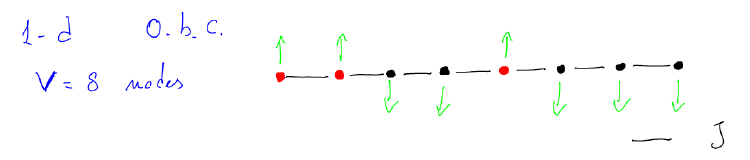
\includegraphics[width=0.7\textwidth]{image016.png}
    \caption{One-dimensional Ising Model with \textbf{open} boundary conditions.\label{fig:obcd1}}
\end{figure}

The partition function is given by:
\begin{align*}
    Z_L(K) &\underset{(\ref{eqn:Z-Is})}{=} 
    \sum_{\{\bm{\sigma}\}}\exp\left( K \sum_{\langle x,y \rangle} \sigma_x \sigma_y \right) =
    \sum_{\sigma_1 = \pm 1} \cdots \sum_{\sigma_{L-1}=\pm 1} \hlc{Yellow}{\sum_{\sigma_L = \pm 1}} e^{K \sigma_1 \sigma_2} e^{K \sigma_2 \sigma_3} \cdots \hlc{Yellow}{e^{K \sigma_{L-1} \sigma_L}} =\\
    &\underset{(a)}{=}  \sum_{\sigma_1 = \pm 1} \cdots \sum_{\sigma_{L-1}=\pm 1} e^{K \sigma_1 \sigma_2} \cdots e^{K \sigma_{L-2} \sigma_{L-1}} 2 \cosh (K \sigma_{L-1})
\end{align*}
where in (a) we summed over the last spin $\sigma_L$. Note that $\cosh$ is even, and so (thanks to our choice of \textit{symmetric} spin-like variables):
\begin{align*}
   2\cosh(K \sigma_{L-1}) = 2 \cosh(\pm K)  = 2 \cosh(K)
\end{align*}
and so:
\begin{align*}
    Z_L(K) &= 2\cosh K  \underbrace{\sum_{\sigma_1 = \pm 1} \cdots \sum_{\sigma_{L-1}=\pm 1} e^{K \sigma_1 \sigma_2} \cdots e^{K \sigma_{L-2} \sigma_{L-1}} }_{Z_{L-1}(K)}  = 2\cosh (K) Z_{L-1}(K)
\end{align*}
Reiterating:
\begin{align*}
    Z_L(K) = (2\cosh K)^L \underset{(\ref{eqn:Z-Is})}{\equiv}  e^{- \beta L f(K)} 
\end{align*}
Taking the logarithm of both sides:
\begin{align*}
    L \ln (2 \cosh K) = -\beta L f(K) \Rightarrow -\beta f(K) = \ln(2\cosh K)
\end{align*}

\begin{figure}[H]
    \centering
    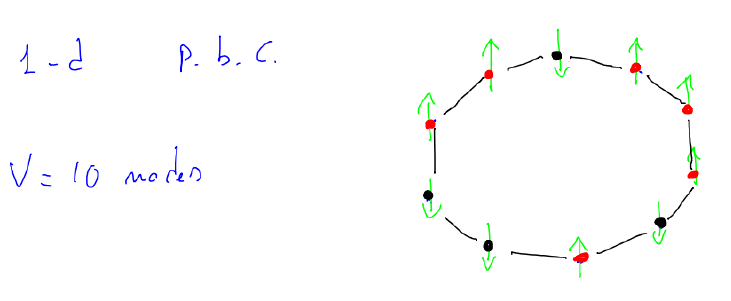
\includegraphics[width=0.7\textwidth]{image017.png}
    \caption{One-dimensional Ising Model with \textbf{periodic} boundary conditions.\label{fig:pbcd1}}
\end{figure}

If we had chosen \textbf{periodic boundary conditions} instead (fig. \ref{fig:pbcd1}) and $h\neq 0$, the partition function would have been:
\begin{align}\label{eqn:Zp}
    Z &\underset{(\ref{eqn:Z-Is})}{=}  \sum_{\{\bm{\sigma}\}} \exp\left(K \sum_{\langle x,y \rangle} \sigma_x \sigma_y + h \sum_x \sigma_x\right)  =\\
    &= \sum_{\sigma_1 \pm 1} \cdots \sum_{\sigma_L = \pm 1} e^{K \sigma_1 \sigma_2} \cdots e^{K \sigma_{L-1} \sigma_L} \hlc{Yellow}{e^{K \sigma_{L} \sigma_{1}} }e^{h \sigma_1} \cdots e^{h \sigma_L}
\end{align} 
Note how the last spin $\sigma_L$ interacts with the first one $\sigma_1$. We can rewrite the spin-spin interactions more compactly as:
\begin{align}\label{eqn:sus1}
    e^{K \sigma_1 \sigma_2} \cdots e^{K \sigma_{L-1} \sigma_L} e^{K \sigma_{L} \sigma_{1}} = \prod_{i=1}^L e^{K \sigma_i \sigma_{i+1}} \qquad \sigma_{L+1} \equiv \sigma_1
\end{align}
With a trick, we can rewrite also the terms $e^{h \sigma_i}$ as a product over \textit{pairs} $(\sigma_i, \sigma_{i+1})$. Thanks to p.b.c., each cell is \textit{connected} to exactly $2$ neighbouring cells (in $d=1$) and so a product over pairs contains the product of \textit{squares} of each node - because each cell is multiplied by itself once for every neighbour: 
\begin{align}\label{eqn:sus2}
    \prod_{i=1}^L e^{h \sigma_i} = \prod_{\langle i, j \rangle} \exp\left(h \frac{\sigma_i + \sigma_j}{2} \right) = \prod_{i=1}^L \exp\left(h \frac{\sigma_i + \sigma_{i+1}}{2} \right) \qquad \sigma_{L+1} \equiv \sigma_1
\end{align}
Substituting (\ref{eqn:sus1}) and (\ref{eqn:sus2}) back in (\ref{eqn:Zp}) leads to:
\begin{align} \label{eqn:Zp2}
    Z = \sum_{\{\bm{\sigma}\}} \prod_{i=1}^L \exp\left(K \sigma_i \sigma_{i+1} + h \frac{\sigma_i + \sigma_{i+1}}{2} \right)
\end{align}
Let's define a \textbf{matrix} \textbf{T}  with entries equal to the factors in (\ref{eqn:Zp2}):
\begin{align}\label{eqn:transfer-elements}
    T_{\sigma \sigma'} \equiv \exp\left(K \sigma \sigma' + h \frac{\sigma + \sigma'}{2} \right)
\end{align}
As $\sigma,\sigma' \in \{\pm 1\}$, \textbf{T} is a $2 \times 2$ matrix:
\begin{align*}
    \textbf{T}  = \begin{blockarray}{l*{2}{c}}
        \begin{block}{l*{2}{>{\scriptstyle}c<{}}}
            & \sigma'=+1 & \sigma'=-1 \\
        \end{block}
        \begin{block}{>{\scriptstyle}r<{}(*{2}{c})}
            \sigma=+1 & e^{K+h} & e^{-K} \\
            \sigma=-1 & e^{-K}   & e^{K-h}\\
        \end{block}
    \end{blockarray}
\end{align*}
\textbf{T} is called the \textbf{transfer matrix} for the $d=1$ Ising Model with periodic boundaries. 

Substituting (\ref{eqn:transfer-elements}) in (\ref{eqn:Zp2}) leads to:
\begin{align*}
    Z &= \sum_{\{\bm{\sigma}\}} \prod_{i=1}^L T_{\sigma_i \sigma_{i+1}} = \sum_{\sigma_1 = \pm 1} \sum_{\sigma_2 = \pm 1} \cdots \sum_{\sigma_{L-1} = \pm 1} \sum_{\sigma_L = \pm 1} T_{\sigma_1 \sigma_2} T_{\sigma_2 \sigma_3} \cdots T_{\sigma_{L-1} \sigma_{L}} T_{\sigma_L \sigma_1} =\\
    &\underset{(a)}{=} 
    \sum_{\sigma_1 = \pm 1} (\underbrace{\textbf{T} \cdot \dots \cdot \textbf{T}}_{L \text{ times}})_{\sigma_1 \sigma_1} =
    \sum_{\sigma_1 = \pm 1} (\textbf{T}^L)_{\sigma_1 \sigma_1} = \operatorname{Tr} \textbf{T}^L 
\end{align*}
In (a), note that all the sums except the first one lead to a \textit{chain} of matrix multiplications:
\begin{align*}
    \sum_a A_{ia} B_{aj} = C_{ij}
\end{align*} 
So, at the end, $Z$ is the sum of the diagonal elements of $\textbf{T}^L$, i.e. its \textbf{trace}.

\medskip

\textbf{T} is symmetric, and so it is diagonalizable, and its eigenvalues are \textbf{real} numbers. Moreover, the trace is basis independent, and so we may compute it in the basis where \textbf{T} is diagonal. Let \textbf{P} be the invertible matrix needed for diagonalizing \textbf{T}, then \textbf{P T P$^{-1}$} $= \operatorname{diag}(\lambda_1, \lambda_2)$, where $\lambda_1$ and $\lambda_2$ are the \textit{eigenvalues} of \textbf{T}. Raising both sides to the $L$-th power, we get:
\begin{align*}
    (\textbf{P}\, \textbf{T}\,\textbf{P}^{-1})^L  = \textbf{P}\,\textbf{T}\,\cancel{\textbf{P}^{-1} \textbf{P}}\,\textbf{T}\,\cancel{\textbf{P}^{-1} \textbf{P}}\cdots \textbf{T}\, \textbf{P}^{-1} = \textbf{P}\,\textbf{T}^L\, \textbf{P}^{-1} = \left(\begin{array}{cc}
    \lambda_1^L & 0 \\ 
    0 & \lambda_2^L
    \end{array}\right)           
\end{align*} 
Then:
\begin{align*}
    \operatorname{Tr}(\textbf{P}\,\textbf{T}^L\,\textbf{P}^{-1}) = \operatorname{Tr}(\textbf{P}^{-1}\,\textbf{P}\,\textbf{T}^L) = \operatorname{Tr}(\textbf{T}^L) =\operatorname{Tr} \left(\begin{array}{cc}
    \lambda_1^L & 0 \\ 
    0 & \lambda_2^L
    \end{array}\right) = \lambda_1^L + \lambda_2^L
\end{align*}
And so:
\begin{align*}
    Z = \operatorname{Tr} \textbf{T}^L = \lambda_1^L + \lambda_2^L  \underset{(\ref{eqn:Z-Is})}{\equiv}  e^{-\beta L f(K,h)}
\end{align*}
Taking the logarithm of both sides:
\begin{align*}
    \ln Z = - \beta L f(K,h) = \ln (\lambda_1^L + \lambda_2^L)
\end{align*}
and dividing by $L$:
\begin{align*}
    \frac{\ln Z}{L} = - \beta f(K,h) = \frac{1}{L} \ln(\lambda_1^L + \lambda_2^L)  
\end{align*}
Suppose (without loss of generality) that $\lambda_1 < \lambda_2$. Then:
\begin{align*}
    -\beta f(K,h) = \frac{1}{L} \ln(\lambda_2^L \Big[1+\left(\frac{\lambda_1}{\lambda_2}\right)^L \Big]) = \frac{1}{\cancel{L}} \cancel{L} \ln \lambda_2 + \frac{1}{L} \ln \left[1+\left(\frac{\lambda_1}{\lambda_2}\right)^L \right]  
\end{align*}
In the thermodynamic limit $L \to \infty$, the larger eigenvalue $\lambda_2$ \textit{dominates}, and $(\lambda_1/\lambda_2)^L \to 0$, so that:
\begin{align}\label{eqn:f-limit}
    -\beta f(K,h) = \ln \lambda_2 + \frac{1}{L} \ln \left[1+\left(\frac{\lambda_1}{\lambda_2}\right)^L \right] \xrightarrow[L \to +\infty]{} \ln \lambda_2
\end{align} 

The eigenvalues can be computed (as usual) as the roots of the \textit{secular} (or \textit{characteristic}) equation:
\begin{align*}
    0 &= \operatorname{det}(\textbf{T} - \lambda \bb{I}) = \operatorname{det} \left|\begin{array}{cc}
    e^{K+h}-\lambda & e^{-K} \\ 
    e^{-K} & e^{K-h}-\lambda
    \end{array}\right| = (e^{K+h} -\lambda)(e^{K-h}-\lambda) - e^{-2K} =\\
    &= \lambda^2 -\lambda e^{K} \frac{e^h + e^{-h}}{\textcolor{Red}{2}}\textcolor{Red}{2} + \frac{e^{2K} - e^{-2K}}{\textcolor{Red}{2}}\textcolor{Red}{2} = \lambda^2 - \lambda e^K \cosh h + 2 \sinh 2K 
\end{align*} 
which are:
\begin{align*}
    \lambda_{1,2} &= e^K \cosh h \mp \sqrt{e^{2K} \cosh^2 h - 2 \sinh 2K} =\\
    &= e^K \cosh h \mp \sqrt{e^{2K} \sinh^2 h + e^{-2K}}
\end{align*}

The \textbf{magnetization} is given by:
\begin{align}\nonumber
    m &\underset{(\ref{eqn:magnetization})}{=}  -\pdv{h} (\beta f) \>\>\overset{\mathclap{L \to \infty}}{\underset{(\ref{eqn:f-limit})}{=}} \>\> \pdv{h} \ln \lambda_2 = \pdv{h} \ln (e^{K} \cosh h + \sqrt{e^{2K} \sinh^2 h + e^{-2K}}) =\\ \nonumber
    &= \frac{1}{e^{K} \cosh h + \sqrt{e^{2K} \sinh^2 h + e^{-2K}}} \left(e^{K} \sinh h + \frac{\cancel{2} e^{2K} \sinh h \cosh h}{\cancel{2} \sqrt{e^{2K} \sinh^2 h + e^{-2K}}} \right) =\\ \nonumber
    &= \frac{1}{e^{K} \cosh h + \sqrt{e^{2K} \sinh^2 h + e^{-2K}}} \frac{\textcolor{Red}{e^K} \sqrt{e^{2K} \sinh^2 h + e^{-2K}} + \textcolor{Red}{e}^{2\textcolor{Red}{K}} \cosh h}{\sqrt{\textcolor{Red}{e^{2K}} \sinh^2 h + \textcolor{Red}{e^{-2K}}}} =\\ \nonumber
    &\underset{(a)}{=}  \frac{1}{\bcancel{e^{K} \cosh h + \sqrt{e^{2K} \sinh^2 h + e^{-2K}}}} \frac{\bcancel{e^K \cosh h + \sqrt{e^{2K} \sinh^2 h + e^{-2K}}}}{\sqrt{\sinh^2 h + e^{-4K}}} =\\
    &=  \frac{\sinh h}{\sqrt{\sinh^2 h + e^{-4K}}} \underset{(b)}{=} \frac{\tanh h}{\sqrt{1 - \frac{1-e^{-4K}}{\cosh^2 h} }} \label{eqn:m-pbc}
\end{align}
where in (a) we divided numerator and denominator by $e^K$, and in (b) by $\cosh h$ and applied the identity $\cosh^2 h - \sinh^2 h = 1 \Rightarrow \sinh^2 h = \cosh^2 h - 1$. 

\medskip

Note that if $K = 0$, and so $J=0$ (non-interacting case), (\ref{eqn:m-pbc}) leads back to $m = \tanh h$, the result we already found in (\ref{eqn:mh}). Moreover, if $K > 0$ (ferromagnetic interaction), $m(K,h) > m(0,h)$ - meaning that spins align more easily to the external field if they can interact with their neighbours.

\medskip

Again, if $h=0$, $m(K,h=0) = 0$, and so the system is unable to magnetize in absence of an external field.

In fact, consider any average spin, e.g. $\langle \sigma_0 \rangle$:
\begin{align*}
    \langle \sigma_0 \rangle = \sum_{\{\bm{\sigma}\}} \exp\left(K \sum_{\langle x,y \rangle} \sigma_x \sigma_y\right)
\end{align*}
For any \textit{finite} system ($L < +\infty$) the sum over all states is a \textit{finite} sum, meaning that it evaluates to some finite number. Moreover, it is \textbf{odd} under the change of variables $\sigma_x \leftrightarrow \sigma_x' = -\sigma_x$:
\begin{align}\label{eqn:symmetry-arg}
    \langle \sigma_0 \rangle = \sum_{\{\bm{\sigma}\}} \exp\left(K \sum_{\langle x,y \rangle} \sigma_x \sigma_y\right)  \sigma_0 = -\sum_{\{\bm{\sigma}\}} \exp\left(K \sum_{\langle x,y \rangle} \sigma_x \sigma_y \right) \sigma_0 = -\langle \sigma_0 \rangle
\end{align} 
and so $\langle \sigma_0 \rangle = 0$. Clearly, this arguments holds for any spin (by translation invariance), and so in general $\langle \sigma_k \rangle = 0$ $\forall k$.

\section{Spontaneous magnetization}
To observe the rise of a \textbf{spontaneous magnetization} (which is the experimental result we wish to model), i.e. a non zero $m$ with no external field ($h=0$), we need to be careful in the \textit{order} of limits. In (\ref{eqn:symmetry-arg}) taking $h = 0$ first leads to $m = 0$ for any finite $V$ - and so also in the thermodynamic limit. The idea is then to \textit{exchange} the two limits:
\begin{align}\label{eqn:break1}
    m(T) = \lim_{h \to 0^+} \lim_{V \to+ \infty} \langle \sigma \rangle_{V,h}
\end{align}
So, first compute the magnetization $\langle \sigma \rangle$ for a finite volume $V$ and in presence of an external field $h \neq 0$. Then perform the thermodynamic limit $V \to \infty$, and only then let go the field $h \to 0^+$. The $m(T)$ so defined is the \textbf{spontaneous magnetization} of the system, and it can be non-zero.

\medskip

The idea is that the \textit{presence} of $h \neq 0$ \textit{breaks} the symmetry ($\bm{\sigma} \leftrightarrow -\bm{\sigma}$) of the system, invalidating argument (\ref{eqn:symmetry-arg}) and thus allowing a spontaneous magnetization.

\medskip

Equivalently, one can break the symmetry without using $h \neq 0$, but by imposing some \textit{fixed} boundary conditions, for example by setting all spins at the boundaries set to $+1$. In this case, the magnetization for a finite volume $V$ is denoted with $\langle \sigma \rangle_V^+$ (\textbf{plus} boundary condition). We can then take the thermodynamic limit:
\begin{align}\label{eqn:break2}
    m(T) = \lim_{V \to +\infty} \langle \sigma \rangle_V^+
\end{align}
The boundary effect will vanish when $V \to \infty$, but it will always break the symmetry of the Hamiltonian ($\bm{\sigma} \leftrightarrow -\bm{\sigma}$).

\medskip

Intuitively, (\ref{eqn:break1}) and (\ref{eqn:break2}) \textit{break} the symmetry in the \q{same direction} (the first with $h>0$, and the latter with $\sigma_i = +1$ at the boundaries), and so we expect them to lead to the same result at the end. For now, no instances in which (\ref{eqn:break1}) and (\ref{eqn:break2}) lead to different results are known.

\medskip

Clearly, we can also consider the limits \textit{from the other direction}, i.e. from $h < 0$, or with \textbf{down} boundary conditions ($\sigma_i = -1$ at the boundaries). The resulting magnetization will be the opposite:
\begin{align*}
    \lim_{h \downarrow 0^+} m(K,h) = \textcolor{Red}{-} \lim_{h \uparrow 0^-} m(K,h)
\end{align*} 

For the Ising Model in $d=1$, $m(T) = 0$. In fact, in computing $m$ in (\ref{eqn:m-pbc}) we first considered the thermodynamic limit $L \to \infty$ for the free energy (\ref{eqn:f-limit}) with $h \neq 0$. Then, taking $h \to 0$ (as already observed), leads to $m = 0$. So, unfortunately, the $d=1$ Ising Model does not suffice to capture the effect of spontaneous magnetization, even when spin-spin interactions are considered. 

\medskip

To observe a phase-transition, we need to find where the free energy $f(K,h)$ is non-analytic. In general, it can be shown that $\forall d > 1$, and $\forall h \neq 0$, $f(K,h)$ is analytic everywhere. The only singular points happen at $h=0$ for $T < T_c$, where $T_c$ is called the \textbf{critical temperature}. 

\begin{figure}[H]
    \centering
    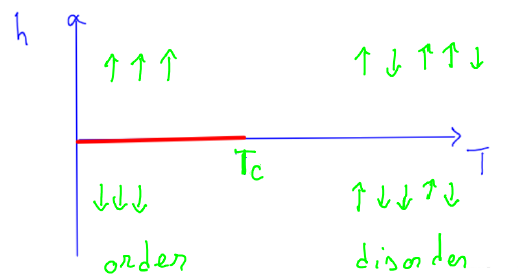
\includegraphics[width=0.7\textwidth]{image018.png} 
    \caption{Phase-diagram showing all parameters $(h,T)$ for which the Ising Model's free energy $f(K,h)$ is non-analytic, which lie on the red segment with $h=0$ and $T=(0,T_c]$. Taking the limit $h \to 0^\pm$ when $T < T_c$ will lead to a non-zero magnetization $m$ (positive if $h \downarrow 0^+$, negative if $h \uparrow 0^-$) - in other words the system \q{spontaneously {organizes}} in absence of an external field (\textbf{ordered phase}). The same limit when $T > T_c$ leads to $m = 0$ - here thermal fluctuations are too high, and the system remains in a random state (\textbf{disordered phase}).\label{fig:non-analytic}}
\end{figure}

\begin{figure}[H]
    \centering
    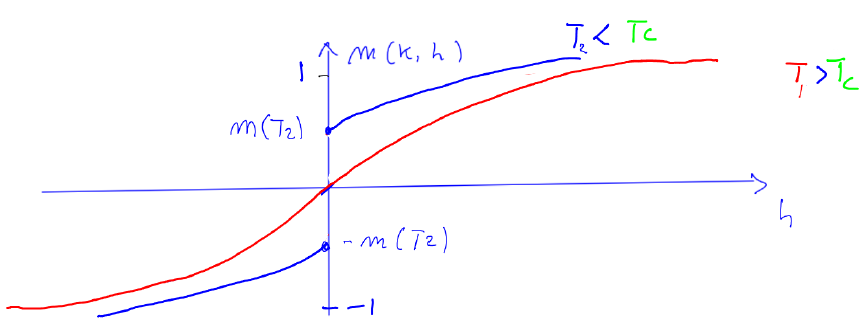
\includegraphics[width=0.7\textwidth]{image019.png}
    \caption{Magnetization at constant temperature $T$ as function of the field strength $h$ (i.e. along a \textit{vertical line} in fig. \ref{fig:m-critical}). If $T > T_c$, as for the red line, the result is the same we obtained in the non-interacting case (fig. \ref{fig:free-spin-m}), or the $d=1$ model. On the other hand, for $T < T_c$ (blue line), a singularity appears at $h=0$, with two possible limits for the magnetization.\label{fig:m-plot}}
\end{figure}

\begin{figure}[H]
    \centering
    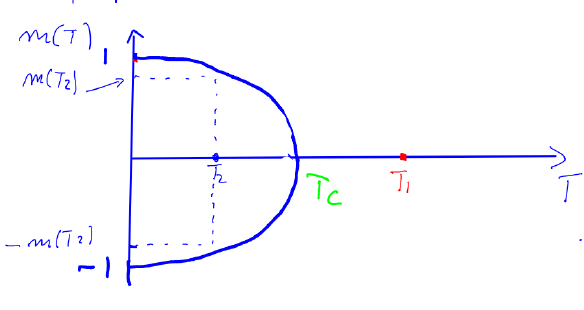
\includegraphics[width=0.7\textwidth]{image020.png}
    \caption{Bifurcation plot for the \textbf{spontaneous magnetization} $m(T)$, i.e. the intercept at $h=0$ of the curves in fig. \ref{fig:m-plot} at various temperatures. For $T > T_c$, all curves $m(h)$ cross the origin, and so lead to no spontaneous magnetization $m(T) = 0$. Conversely, for $T < T_c$, two opposite values of $m(T)$ are possible, depending on the taken limit $h \to 0^\pm$. Note that the region \q{inside the arc} is not reachable (\textbf{unphysical region}): for example at $T = T_2$ it is impossible to obtain a magnetization $|m| < |m(T_2)|$. \label{fig:spont-m}}
\end{figure}



\begin{figure}[H]
    \centering
    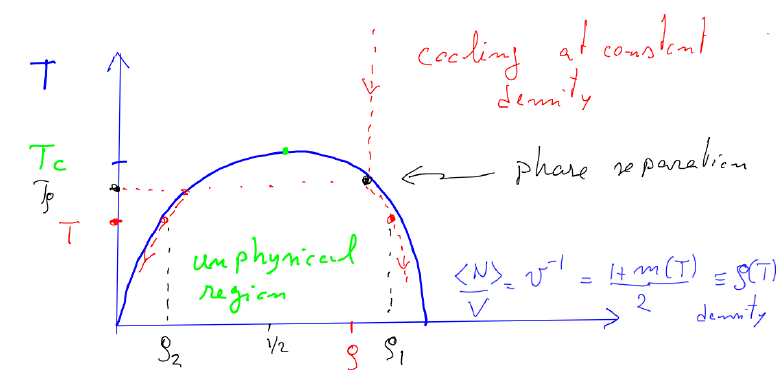
\includegraphics[width=0.7\textwidth]{image021.png}
    \caption{The analogue of the magnetization $m$ in the lattice gas is the \textbf{density} $\rho = v^{-1} = \langle N \rangle /V = (1+m(T))/2$. \label{fig:lattice-critical}} %Mathematically derive the shift and rotation of that curve
\end{figure}

Consider the lattice gas model, with a fraction $\rho$ of occupied cells. Suppose we want to keep $\langle N \rangle$ fixed. This can be done by changing the chemical potential, which is the conjugate variable to $N$, and in the lattice gas model takes the role the external magnetic field had in the ferromagnetic Ising Model (in fact the magnetic field $b$ is a function of $\ln z$, which contains $\mu$).

Lowering the temperature (moving along the red dashed line), to keep $\rho$ fixed, $\mu$ has to change. When it reaches the blue curve, a \textit{phase separation} is observed, and the gas divides in two parts: one of low density $\rho_2$, and one with higher density $\rho_1$. Graphically, until the blue curve is reached, the gas is \q{well mixed}: every region has almost the same density. After, it is divided in mostly empty regions and very dense regions (fig. \ref{fig:fluid-sep}).

\begin{figure}[H]
    \centering
    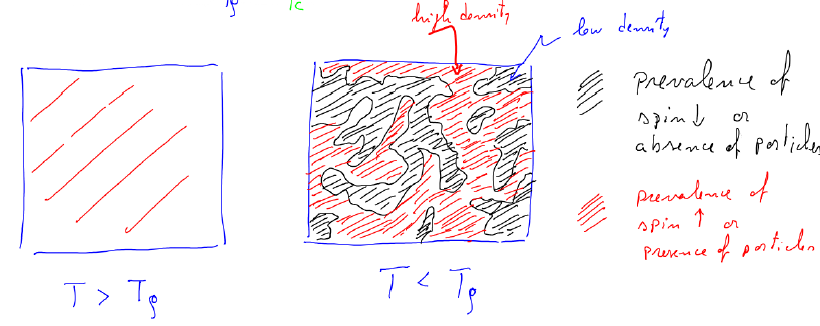
\includegraphics[width=0.7\textwidth]{image022.png}
    \caption{The lattice gas is well-mixed for $T > T_\rho$ (left figure), but separates in two phases with different densities for $T < T_\rho$.\label{fig:fluid-sep}}
\end{figure}

Let $f_i$ be the fraction of volume occupied by the fluid with density $\rho_i$ satisfies:
\begin{align*}
    f_1 \rho_1 + f_2 \rho_2 = \rho
\end{align*}
and $\rho$ is fixed and remains constant. Also $f_1 + f_2 = 1$. Then:
\begin{align*}
    \rho_1 = \frac{1+m(T)}{2}; \qquad \rho_2 = \frac{1-m(T)}{2}  
\end{align*}
leading to:
\begin{align*}
    f_1(T) = 1-f_2(T) = \frac{1}{2} \left(1+\frac{2 \rho -1}{m(T)} \right) 
\end{align*}

%Last 8 minutes
\begin{align*}
    \rho = \begin{cases}
        \frac{1+m(T_\rho)}{2} & \rho > \frac{1}{2}\\
        \frac{1-m(T_\rho)}{2} & \rho < \frac{1}{2}    
    \end{cases}
\end{align*}

$T_\rho$ is defined as the temperature at which the red dashed line intercepts the blue curve, i.e. at which phase separation occurs. 



\begin{figure}[H]
    \centering
    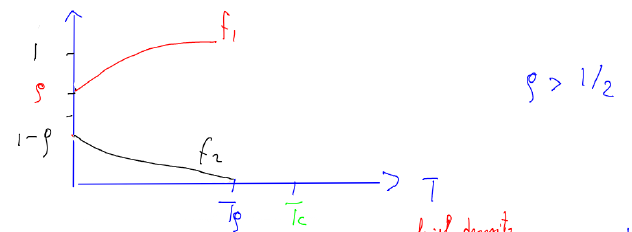
\includegraphics[width=0.7\textwidth]{image023.png}
    \caption{\label{fig:fluid-phases}}
\end{figure}

Spinoidal decomposition: try to enter in the unphysical region by rapidly cooling the gas. 

\end{document}
